% This file was created with tikzplotlib v0.10.1.
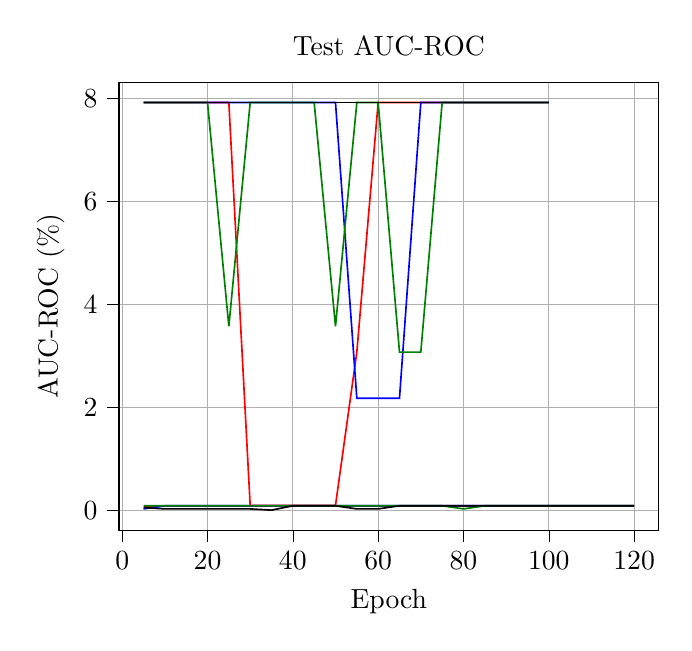
\begin{tikzpicture}

\definecolor{darkgray176}{RGB}{176,176,176}
\definecolor{green}{RGB}{0,128,0}

\begin{axis}[
tick align=outside,
tick pos=left,
title={Test AUC-ROC},
x grid style={darkgray176},
xlabel={Epoch},
xmajorgrids,
xmin=-0.75, xmax=125.75,
xtick style={color=black},
y grid style={darkgray176},
ylabel={AUC-ROC (\%)},
ymajorgrids,
ymin=-0.393790903365372, ymax=8.31590310207331,
ytick style={color=black}
]
\addplot [semithick, red]
table {%
5 7.92000792000792
10 7.92000792000792
15 7.92000792000792
20 7.92000792000792
25 7.92000792000792
30 0.0945291267871913
35 0.0945291267871913
40 0.0945291267871913
45 0.0945291267871913
50 0.0945291267871913
55 3.07265549983997
60 7.92000792000792
65 7.92000792000792
70 7.92000792000792
75 7.92000792000792
80 7.92000792000792
85 7.92000792000792
90 7.92000792000792
95 7.92000792000792
100 7.92000792000792
};
\addplot [semithick, blue]
table {%
5 7.92000792000792
10 7.92000792000792
15 7.92000792000792
20 7.92000792000792
25 7.92000792000792
30 7.92000792000792
35 7.92000792000792
40 7.92000792000792
45 7.92000792000792
50 7.92000792000792
55 2.17604178000218
60 2.17604178000218
65 2.17604178000218
70 7.92000792000792
75 7.92000792000792
80 7.92000792000792
85 7.92000792000792
90 7.92000792000792
95 7.92000792000792
100 7.92000792000792
};
\addplot [semithick, green]
table {%
5 7.92000792000792
10 7.92000792000792
15 7.92000792000792
20 7.92000792000792
25 3.57142857142857
30 7.92000792000792
35 7.92000792000792
40 7.92000792000792
45 7.92000792000792
50 3.57142857142857
55 7.92000792000792
60 7.92000792000792
65 3.07265549983997
70 3.07265549983997
75 7.92000792000792
80 7.92000792000792
85 7.92000792000792
90 7.92000792000792
95 7.92000792000792
100 7.92000792000792
};
\addplot [semithick, black]
table {%
5 7.92000792000792
10 7.92000792000792
15 7.92000792000792
20 7.92000792000792
25 7.92000792000792
30 7.92000792000792
35 7.92000792000792
40 7.92000792000792
45 7.92000792000792
50 7.92000792000792
55 7.92000792000792
60 7.92000792000792
65 7.92000792000792
70 7.92000792000792
75 7.92000792000792
80 7.92000792000792
85 7.92000792000792
90 7.92000792000792
95 7.92000792000792
100 7.92000792000792
};
\addplot [semithick, red]
table {%
5 0.0865384615384615
10 0.0865384615384615
15 0.0865384615384615
20 0.0865384615384615
25 0.0865384615384615
30 0.0865384615384615
35 0.0865384615384615
40 0.0865384615384615
45 0.0865384615384615
50 0.0865384615384615
55 0.0865384615384615
60 0.0865384615384615
65 0.0865384615384615
70 0.0865384615384615
75 0.0865384615384615
80 0.0865384615384615
85 0.0865384615384615
90 0.0865384615384615
95 0.0865384615384615
100 0.0865384615384615
105 0.0865384615384615
110 0.0865384615384615
115 0.0865384615384615
120 0.0865384615384615
};
\addplot [semithick, blue]
table {%
5 0.0260719672484378
10 0.0865384615384615
15 0.0865384615384615
20 0.0865384615384615
25 0.0865384615384615
30 0.0865384615384615
35 0.0865384615384615
40 0.0865384615384615
45 0.0865384615384615
50 0.0865384615384615
55 0.0865384615384615
60 0.0865384615384615
65 0.0865384615384615
70 0.0865384615384615
75 0.0865384615384615
80 0.0865384615384615
85 0.0865384615384615
90 0.0865384615384615
95 0.0865384615384615
100 0.0865384615384615
105 0.0865384615384615
110 0.0865384615384615
115 0.0865384615384615
120 0.0865384615384615
};
\addplot [semithick, green]
table {%
5 0.0865384615384615
10 0.0865384615384615
15 0.0865384615384615
20 0.0865384615384615
25 0.0865384615384615
30 0.0865384615384615
35 0.0865384615384615
40 0.0865384615384615
45 0.0865384615384615
50 0.0865384615384615
55 0.0865384615384615
60 0.0865384615384615
65 0.0865384615384615
70 0.0865384615384615
75 0.0865384615384615
80 0.0260719672484378
85 0.0865384615384615
90 0.0865384615384615
95 0.0865384615384615
100 0.0865384615384615
105 0.0865384615384615
110 0.0865384615384615
115 0.0865384615384615
120 0.0865384615384615
};
\addplot [semithick, black]
table {%
5 0.0525829310876039
10 0.0260719672484378
15 0.0260719672484378
20 0.0260719672484378
25 0.0260719672484378
30 0.0260719672484378
35 0.0021042787000233
40 0.0865384615384615
45 0.0865384615384615
50 0.0865384615384615
55 0.0260719672484378
60 0.0260719672484378
65 0.0865384615384615
70 0.0865384615384615
75 0.0865384615384615
80 0.0865384615384615
85 0.0865384615384615
90 0.0865384615384615
95 0.0865384615384615
100 0.0865384615384615
105 0.0865384615384615
110 0.0865384615384615
115 0.0865384615384615
120 0.0865384615384615
};
\end{axis}

\end{tikzpicture}
